%
% Main thesis LaTeX file. We use the REPORT style format
% instead of article for most technical papers
%
%
\documentclass[12pt,fleqn]{article}

%%%%%%%%%%%%%%%%%%%%%%%%%%%%%%%%%%%%%%%%%%%%%%%%%%%%%%%%%%%%%%%%%%%%
%
% list the set of packages we use for various aspects of 
% the thesis format
%
\usepackage{layout}
\usepackage[utf8]{inputenc}
\usepackage{setspace}

\usepackage{subfigure}
\usepackage{epsfig}
\usepackage{float}
\usepackage{floatflt}
\usepackage{listings}
\usepackage{palatino}
\usepackage{verbatim}
\usepackage{footnpag}
\usepackage{caption}
\usepackage[mathcal, mathbf]{euler}
\usepackage{amsmath}
\usepackage{amstext}
\usepackage{color}
\usepackage{xcolor}
\usepackage{graphicx}


%%%%%%%%%%%%%%%%%%%%%%%%%%%%%%%%%%%%%%%%%%%%%%%%%%%%%%%%%%%%%%%%%%%%
%
% include two local LaTeX source files that establish the
% thesis layout and the set of additional commands we find
% useful for creating the text.
%
\input{layout}
\input{newcommands}
\input{outline_support}


\newcommand{\Organization}{School of Computer Engineering}

\title{CE2004: Circuits \& Signal Analysis Part 2}

\author{
  Lu Shengliang \\
  SLU001\\
  \Organization{} \\
  \vspace*{-10mm} \\
  Nanyang Technological University \\
  \vspace*{-10mm} \\
  SLU001@e.ntu.edu.sg
}

%
% This begins the actual lab report
%
\renewcommand{\OutlineLevel}{2}

\begin{document}
\lstset{language=Scilab}
\maketitle

\begin{abstract}
\ls{1}
\emph{lab 4}: Use \emph{Scilab} software package to demonstrate how signals can be simulated. \textbf{\emph{Step}}, \textbf{\emph{Rectangular}}, \textbf{\emph{Sinusoidal}}, \textbf{\emph{delta}} functions and \textbf{\emph{Square}} series were conducted.   
\ls{1.2}
\end{abstract}

\ls{1.2}

\section{Defining and Plotting Step Functions}
define a step function called \emph{\textbf{step(t)}} that is equal to 1 when t $\geq$ 0, and is equal to 0 when t \textless{} 0.
\subsection{Step function u(t)}
\begin{lstlisting}[frame=single]
function y = step(t)
    y = round((sign(t) + 1) / 2)
endfunction
\end{lstlisting}
\begin{figure}[H]
\centering
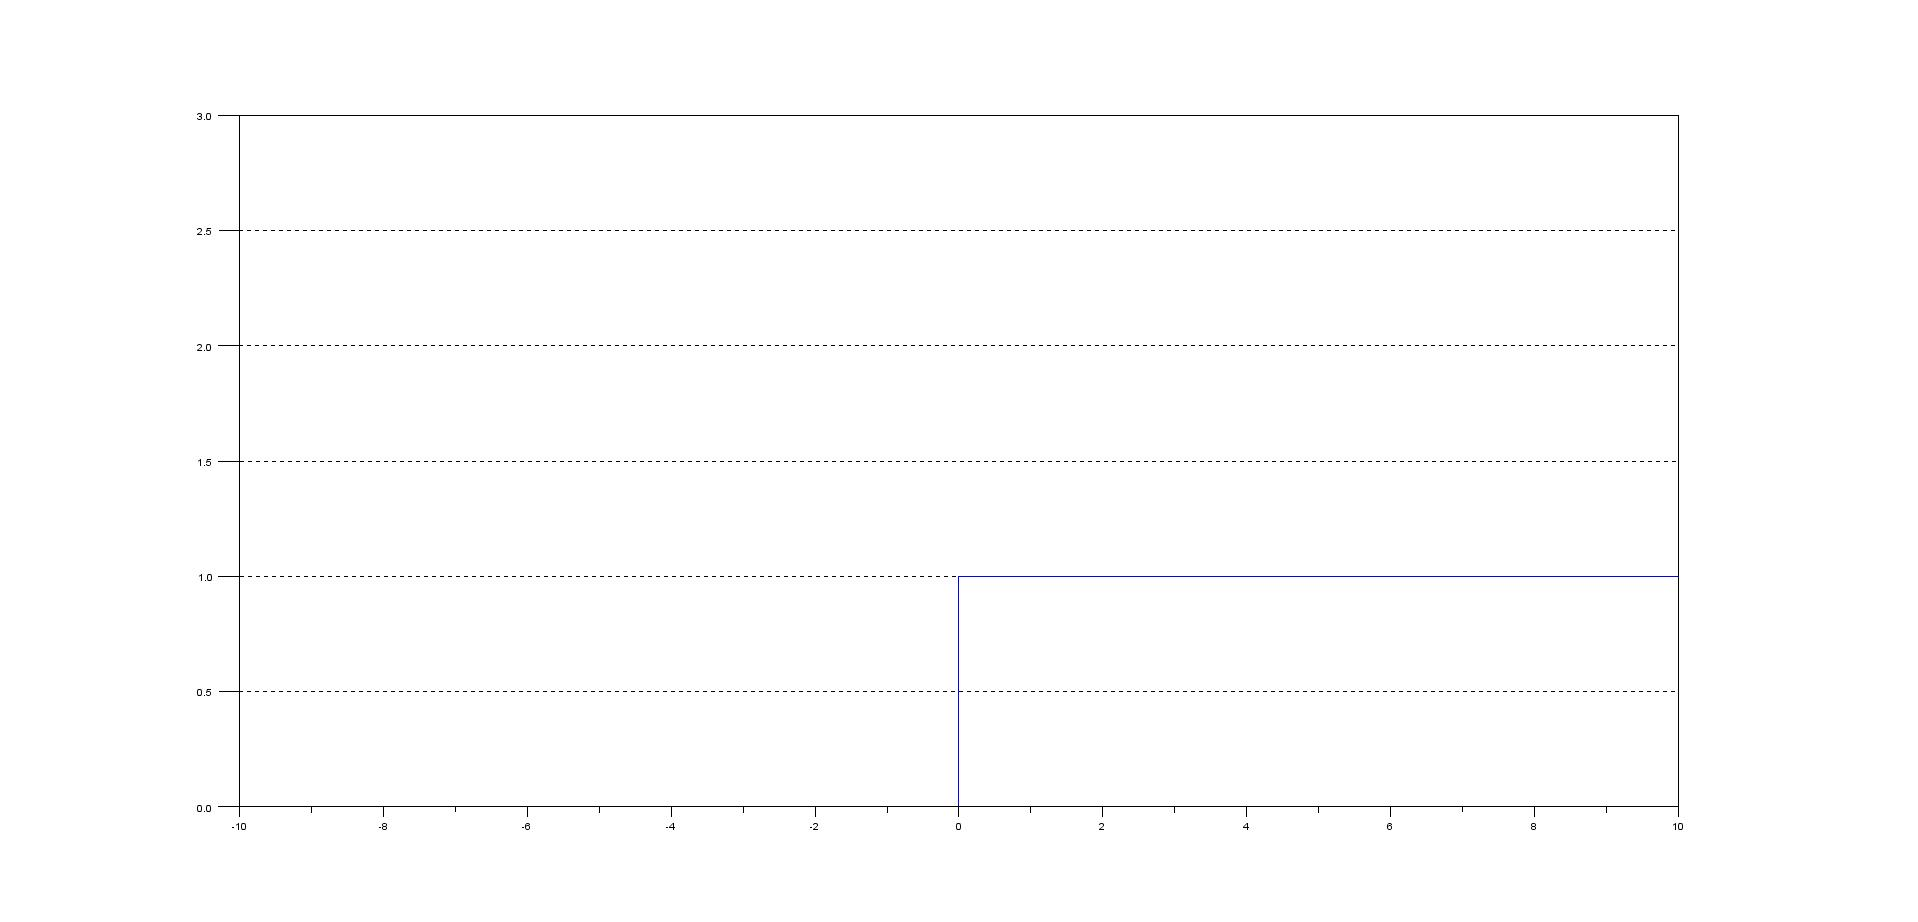
\includegraphics[width=\textwidth]{u(t).jpg}
\caption{step function $u(t)$}
\end{figure}

\subsection{Plotting of different step functions}
\begin{lstlisting}[frame=single]
plot(t, step(t - 1))
\end{lstlisting}
\begin{figure}[H]
\centering
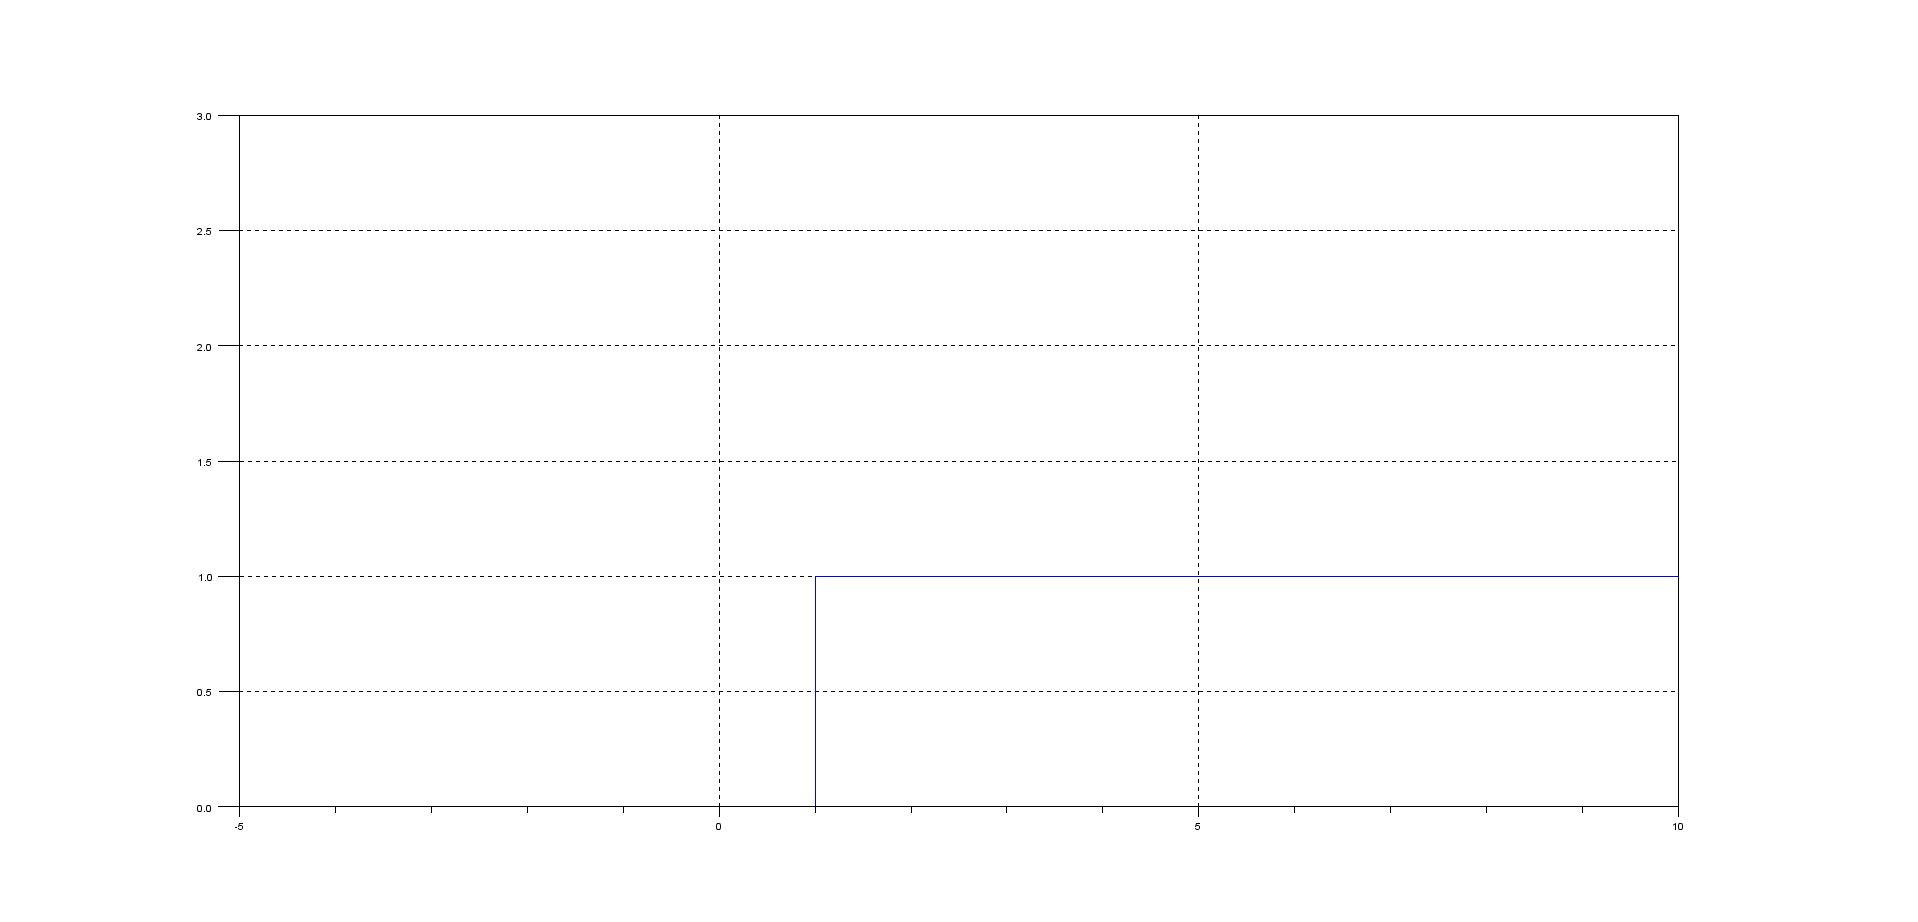
\includegraphics[width=\textwidth]{u(t-1).jpg}
\caption{$u(t-1)$}
\end{figure}

\begin{lstlisting}[frame=single]
plot(t, 2 * u(t + 2))
\end{lstlisting}
\begin{figure}[H]
\centering
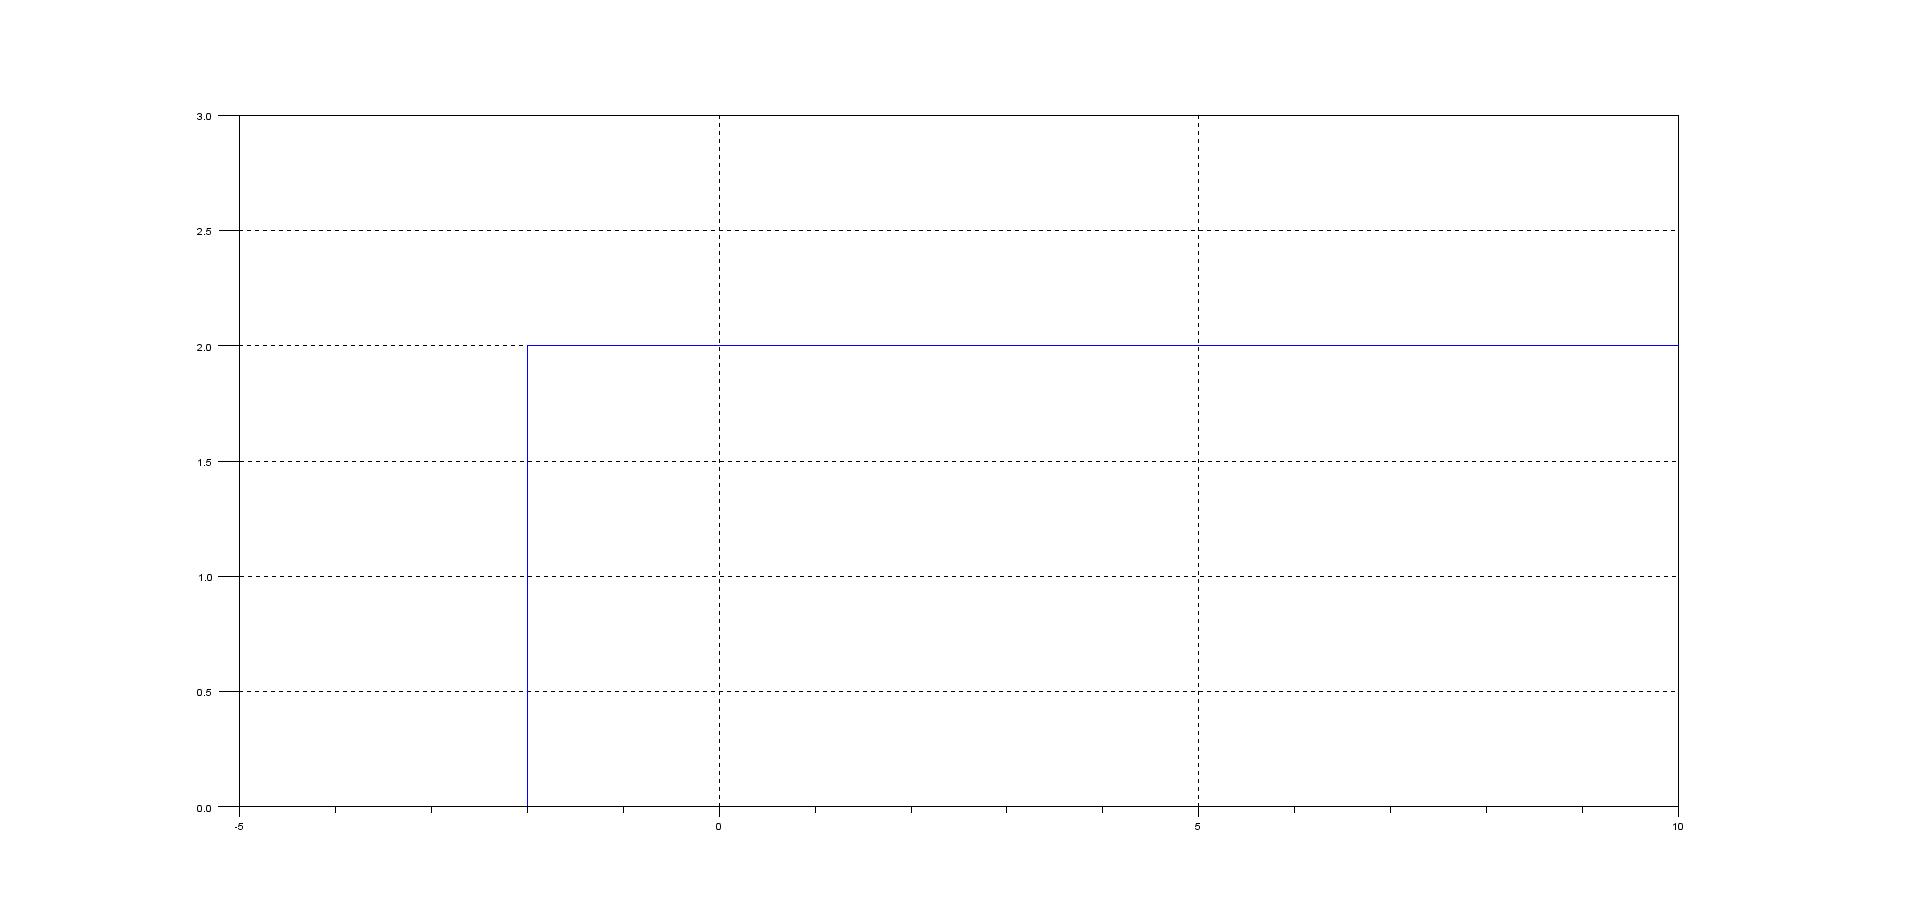
\includegraphics[width=\textwidth]{2xu(t+2).jpg}
\caption{$2*u(t+2)$}
\end{figure}

\begin{lstlisting}[frame=single]
plot(t, u(t + 1) - u(t - 1))
\end{lstlisting}
\begin{figure}[H]
\centering
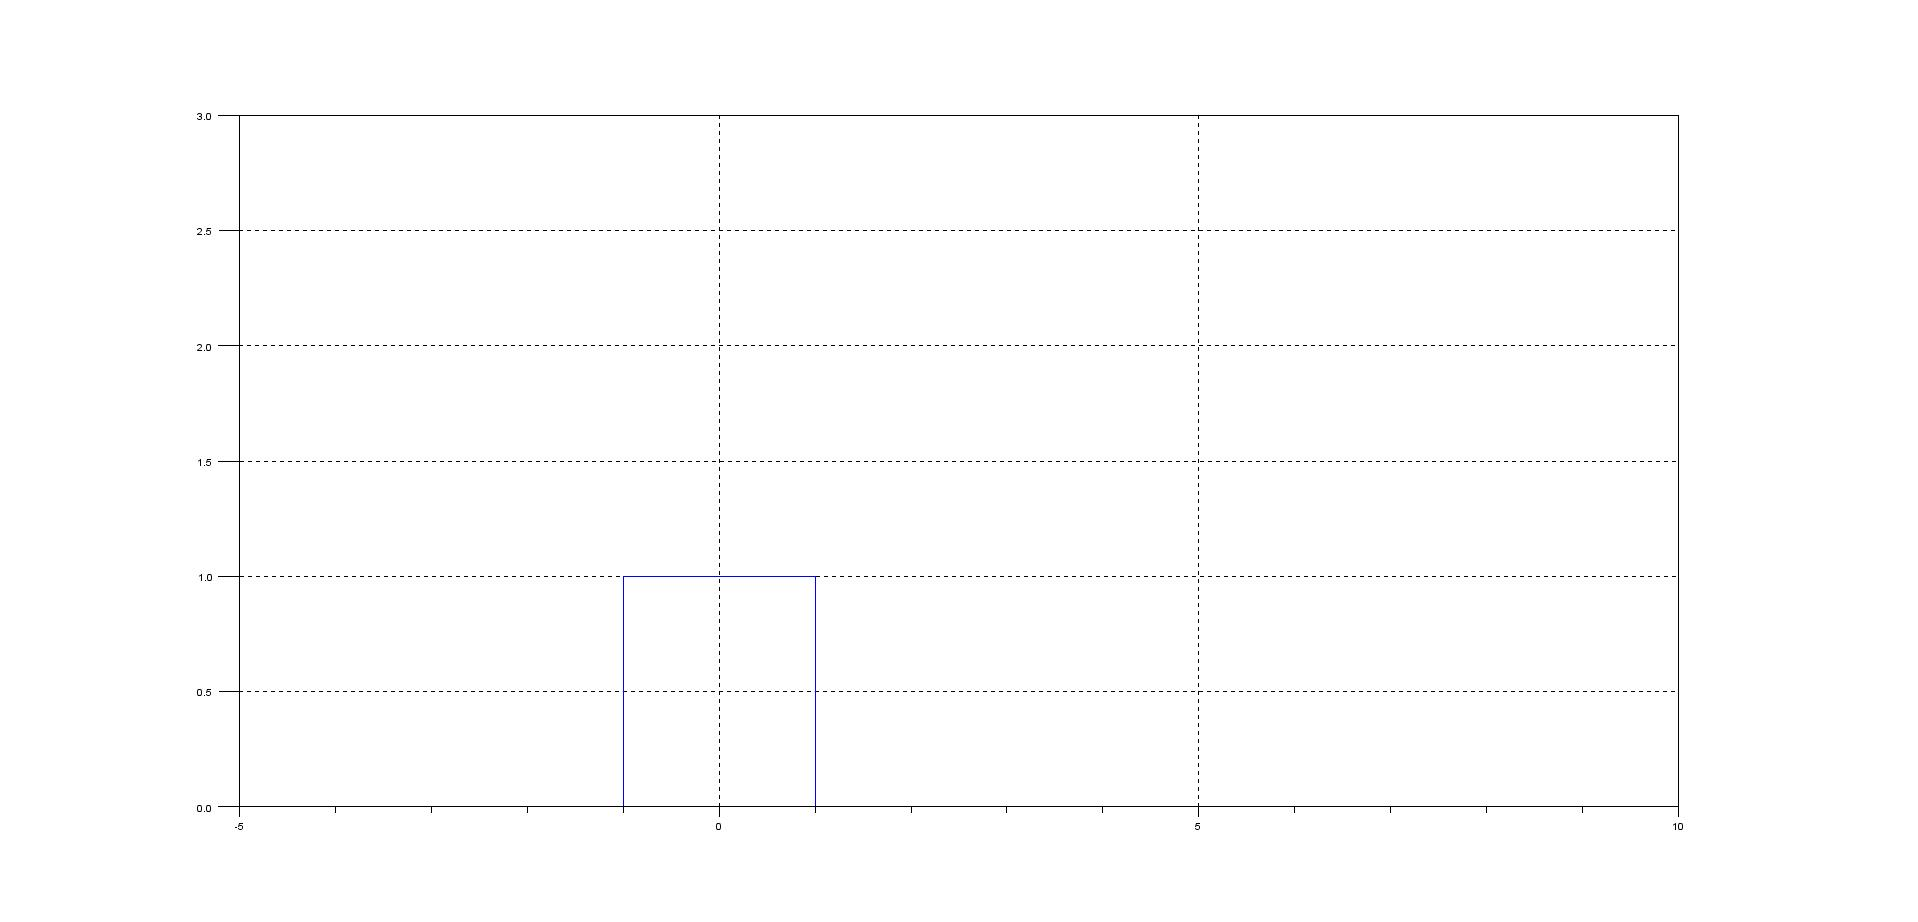
\includegraphics[width=\textwidth]{u(t+1)-u(t-1).jpg}
\caption{$u(t+1)-u(t-1)$}
\end{figure}
\subsection{Question 5.1}
\textbf{Question:}\\
Save the plots and comment on the observed shapes of the signals.\\
\textbf{Answer:}\\
The step function was generated by built-in \emph{\textbf{sign()}} function. It returns 1 when t $\geq$ 0, otherwise 0. \\
So $u(t-1)$ is basically step function after shifting right 1 unit on x-axis. \\
$2*u(t+2)$ is step function shifting 2 unit left and then doubling the height of it. \\
$u(t+1)-u(t-1)$ is actually the way of generating $\Pi$ function. The difference is that its graphic width is 2 rather than $\Pi$ function's one-unit width.

%================================================
\section{Defining and Plotting Rectangular Functions}
Rectangular function(or $\Pi$ function) equals to 1 when -0.5 $\leq$ t $\leq$ 0.5 and equals to 0 otherwise. Use the previously defined step function to generate a square function $\Pi(t)$.
\subsection{Square function pi(t)}
\begin{lstlisting}[frame=single]
function y = pi(t)
    y = step(t + 0.5) - step(t - 0.5)
endfunction
\end{lstlisting}
\begin{figure}[H]
\centering
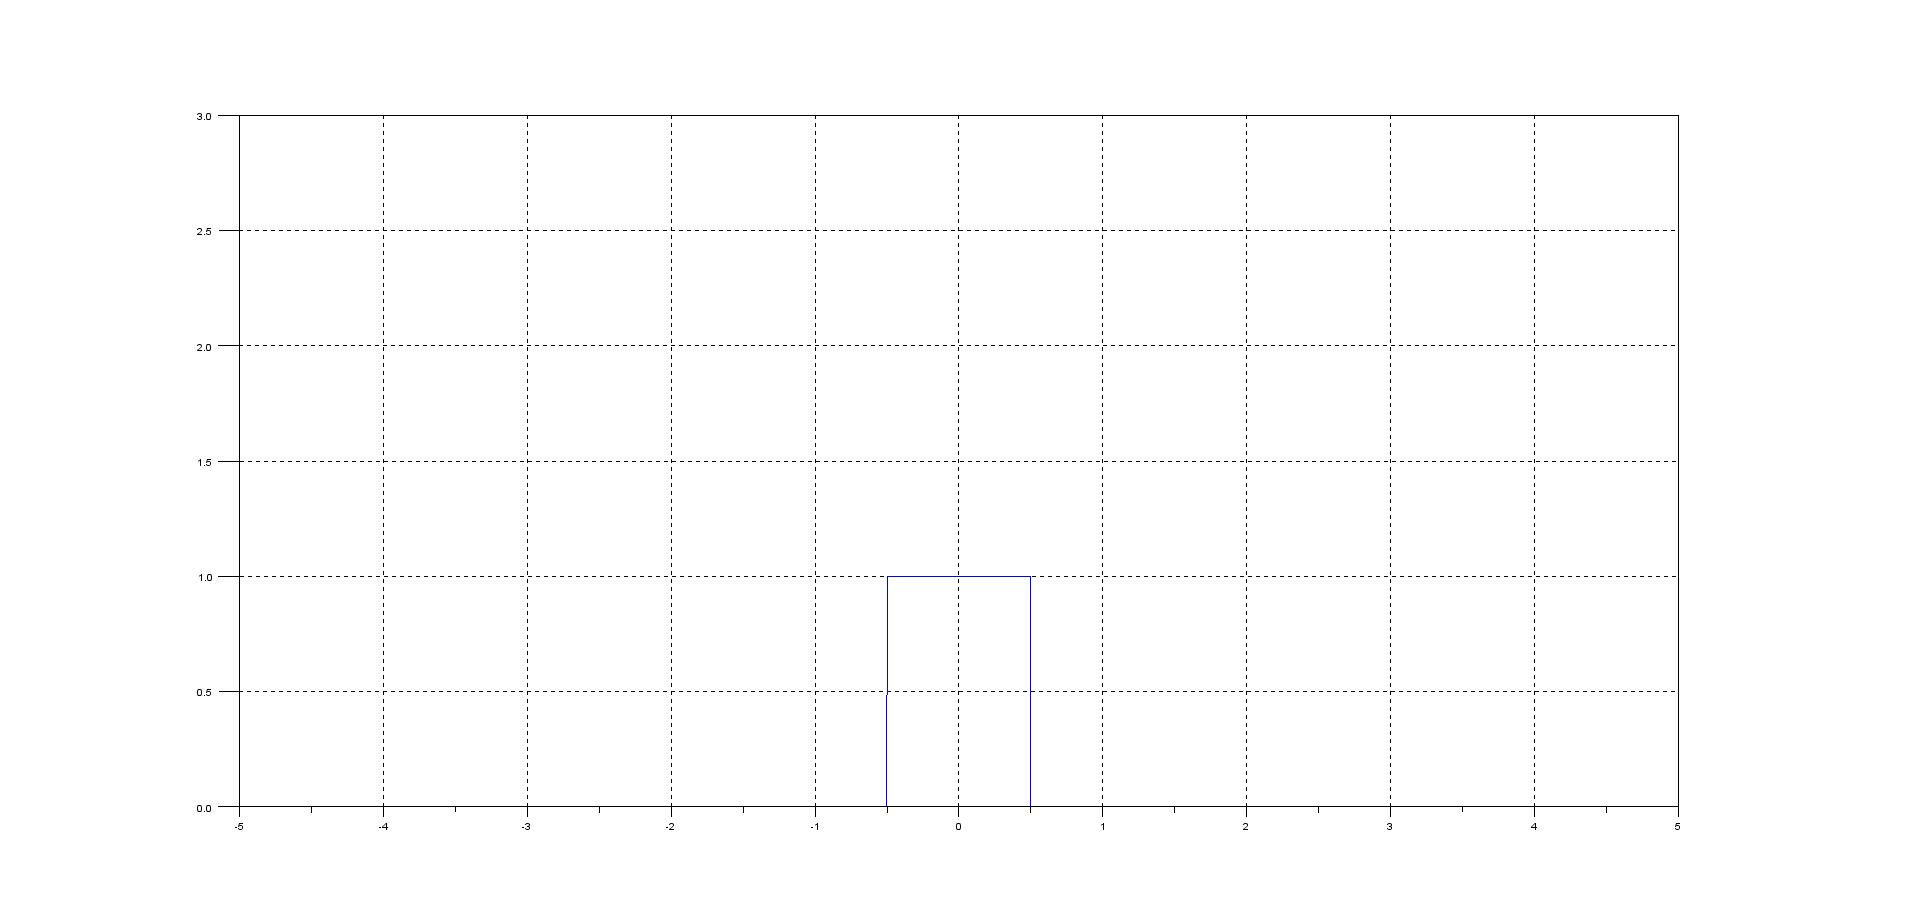
\includegraphics[width=\textwidth]{pi(t).jpg}
\caption{square function $\Pi(t)$}
\end{figure}

\begin{lstlisting}[frame=single]
plot(t, pi(2 * t - 1))
\end{lstlisting}
\begin{figure}[H]
\centering
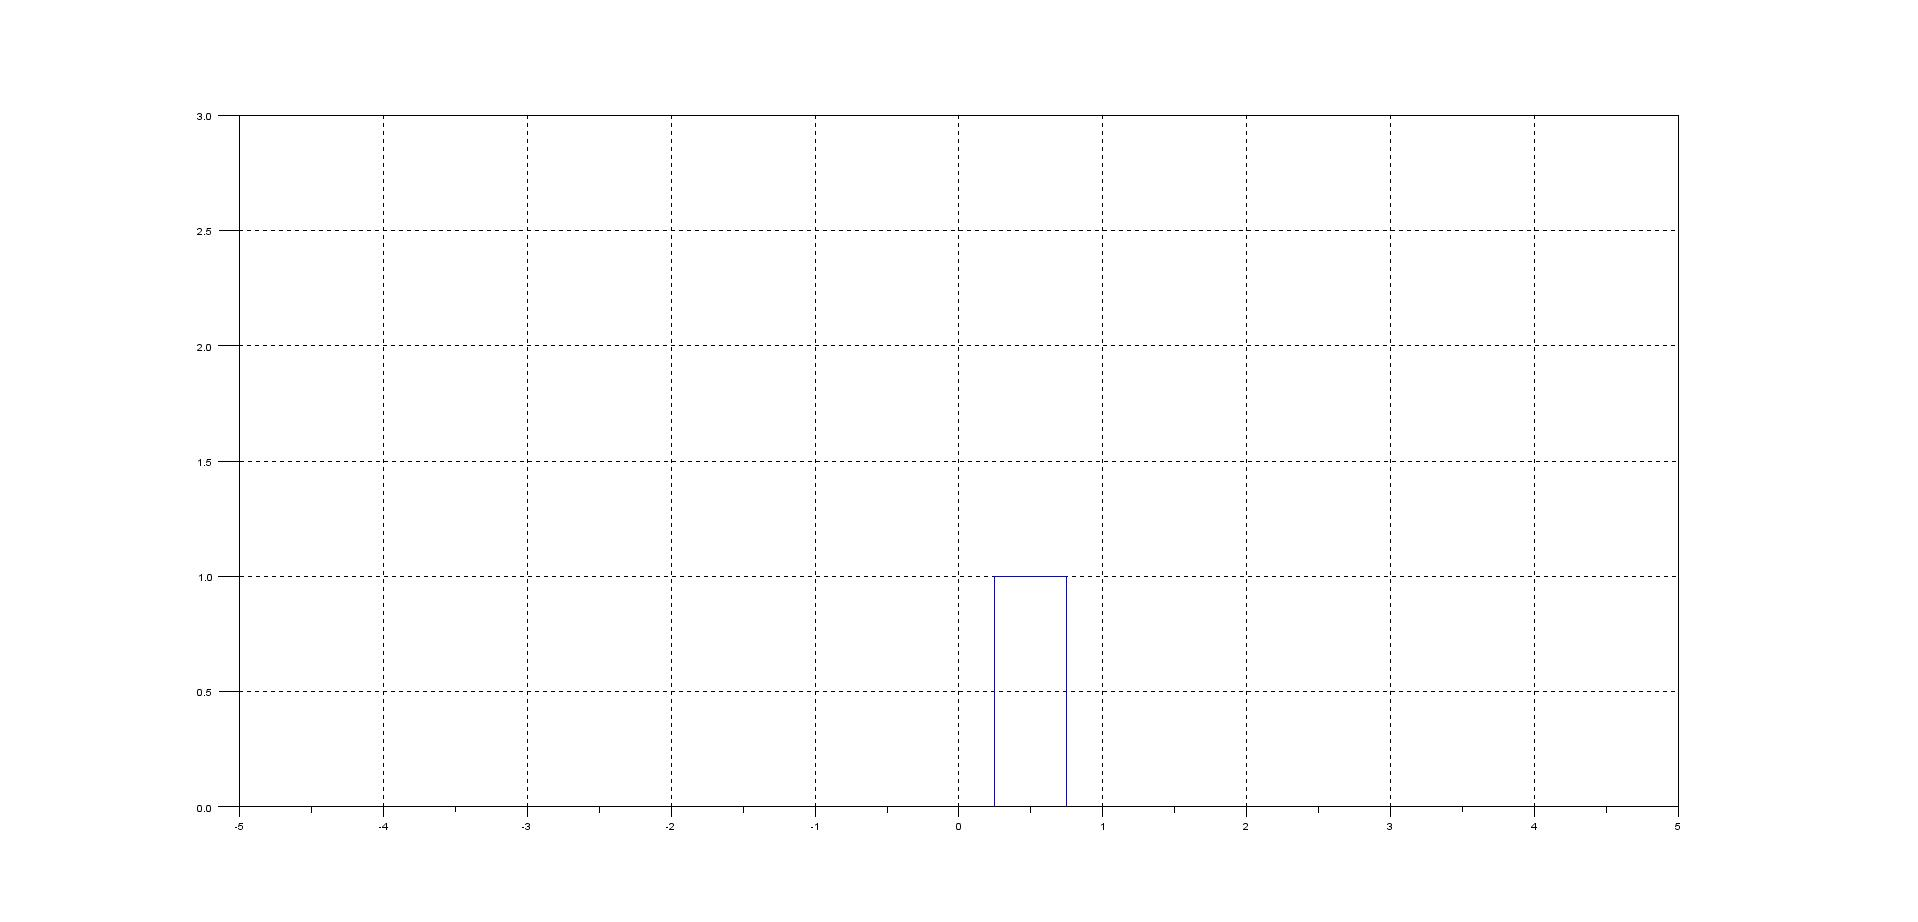
\includegraphics[width=\textwidth]{pi(2t-1).jpg}
\caption{$\Pi(2t-1)$}
\end{figure}

\begin{lstlisting}[frame=single]
plot(t, 1.5 * pi(-6 * t + 5))
\end{lstlisting}
\begin{figure}[H]
\centering
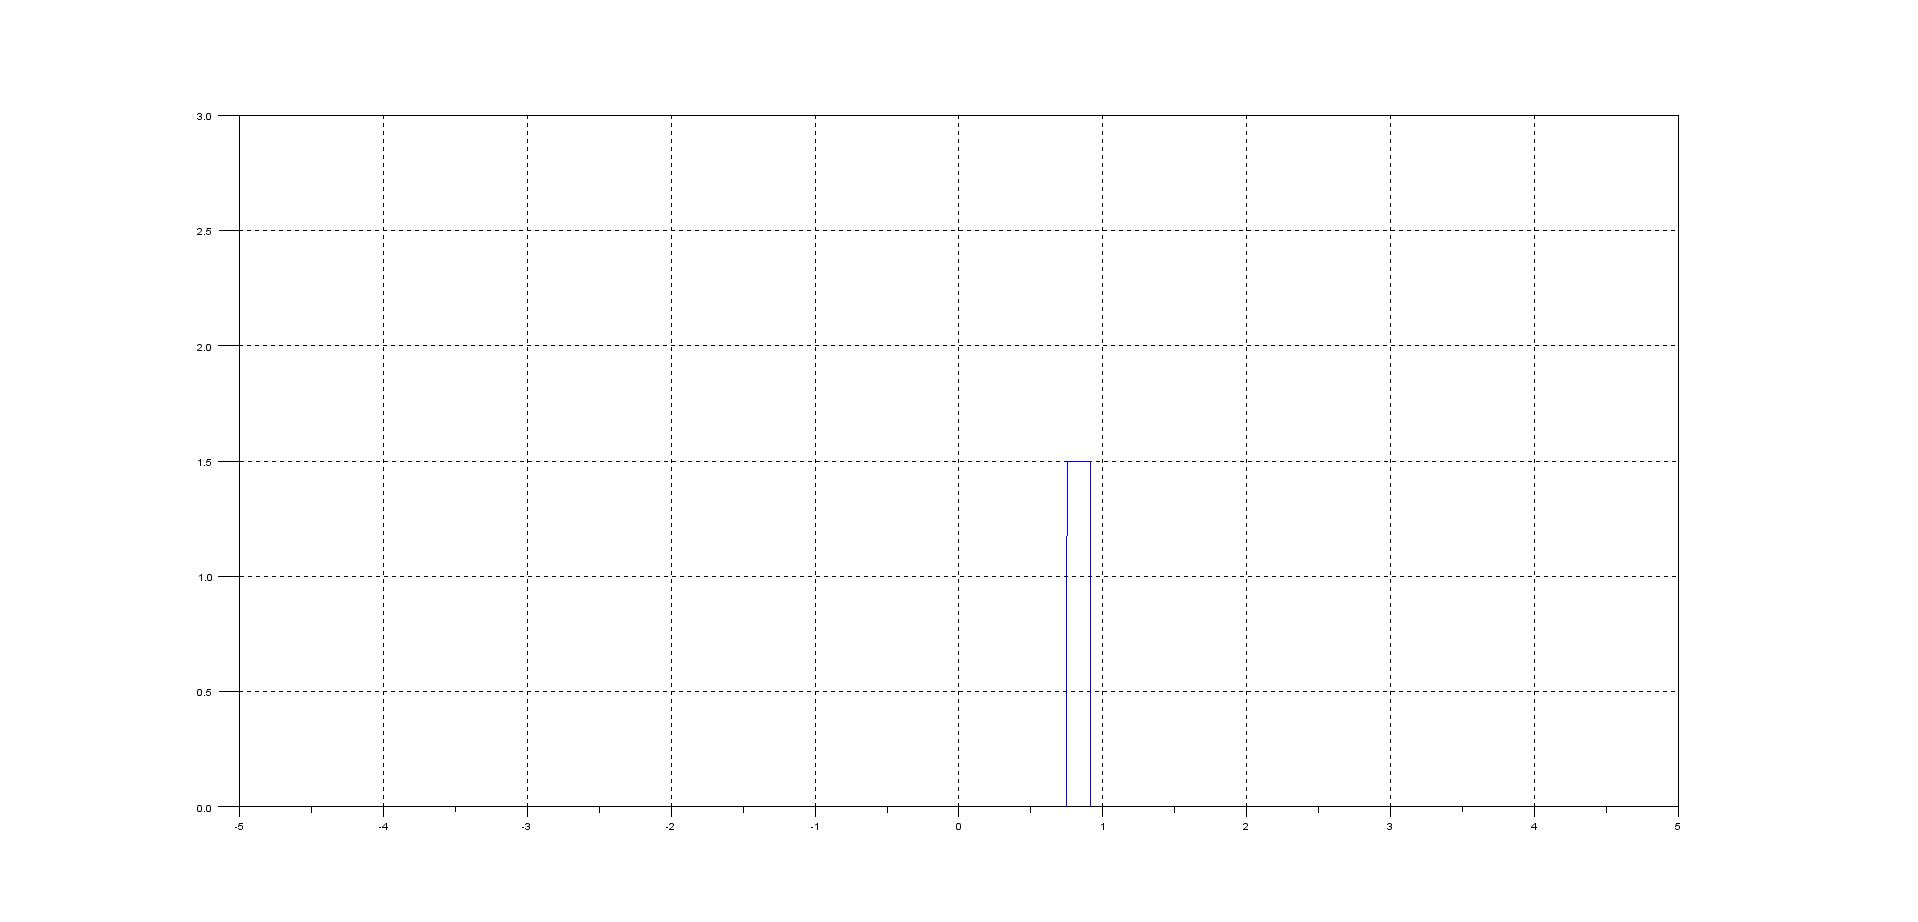
\includegraphics[width=\textwidth]{15Pi(-6t+5).jpg}
\caption{$1.5*\Pi(-6t+5)$}
\end{figure}

\begin{lstlisting}[frame=single]
function y = Pic(t)
    y = Pi(0.5*t-2) + 2*Pi(0.5*t-1) + 3*Pi(0.5*t) 
      + 2*Pi(0.5*t+1) + Pi(0.5*t+2)
endfunction
\end{lstlisting}
\begin{figure}[H]
\centering
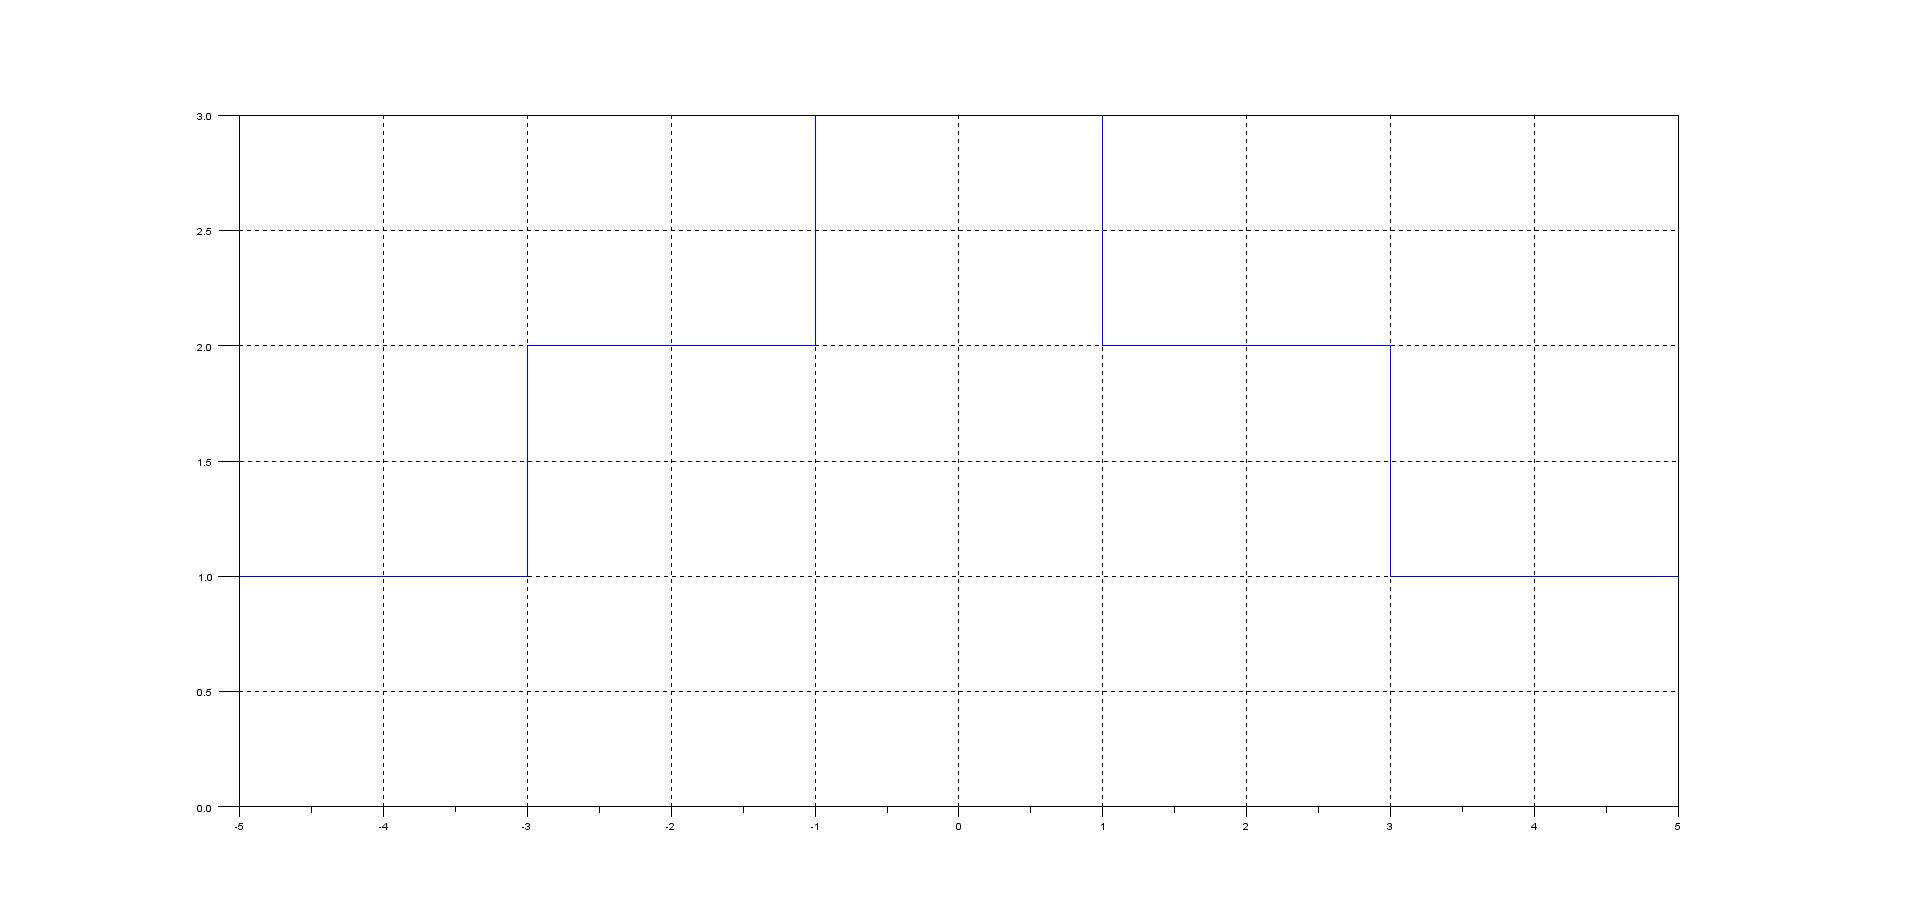
\includegraphics[width=\textwidth]{pic.jpg}
\caption{$\Pi(0.5t-2)+2\Pi(0.5t-1)+3\Pi(0.5t)+2\Pi(0.5t+1)+\Pi(0.5t+2)$}
\end{figure}

\subsection{Question 5.2}
\textbf{Question:}\\
Save the plots and comment on the observed shapes of the signals.\\
\textbf{Answer:}\\
The rectangular function was generated by \emph{\textbf{step}} function. It returns 1 when when -0.5 $\leq$ t $\leq$ 0.5 and is equal to 0 otherwise.\\
So $\Pi(2t-1)$ is basically rectangular function shifting right by 1 unit on x-axis and compressing a half on x-axis.\\
1.5 * $\Pi(-6t+5)$ is rectangular function shifting right $\frac{5}{6}$ unit on x-axis and compressing by 6, then increasing the height of sign to 1.5 times.\\
The last one is actually the combination of 5 different heights $\Pi$ functions after doubling their widths. 

%==================================================
\section{Defining Sinusoidal Signals and Converting Them into Sounds}
Use built-in sine function \emph{\textbf{sin(t)}} to generate the following signals with 0.0001 sampling interval and save them using \emph{\textbf{savewave()}} command.
\subsection{2-second duration middle C}
2-second duration signal corresponding to a sine wave with frequency 261.63Hz
\begin{lstlisting}[frame=single]
function y = wavA(t)
    y = sin(261.63*2*%pi*t)
endfunction
t = 0 : 0.0001 : 4.41
\end{lstlisting}
\begin{figure}[H]
\centering
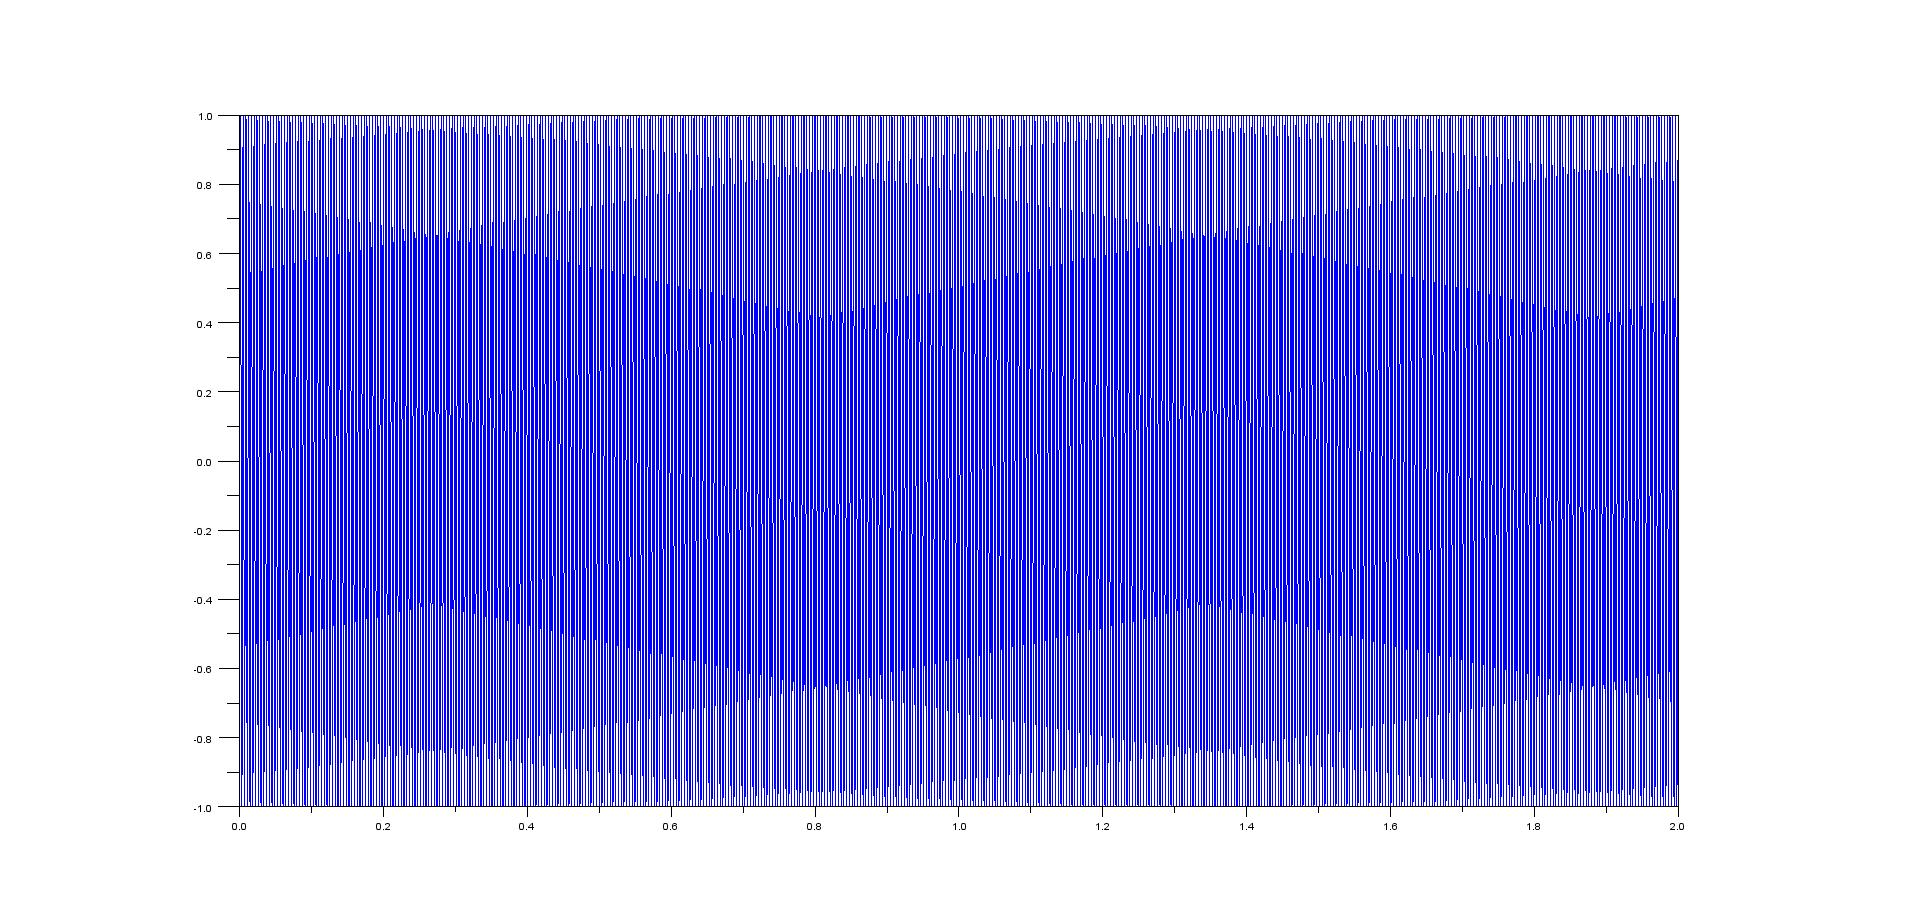
\includegraphics[width=\textwidth]{3a.jpg}
\caption{middle C}
\end{figure}
Because 22050 is the default value of number of sample per second, in order to get a 2-second duration sound, the length of t should be 4.41.
\begin{gather}
rangeT = 22050 sample/second \times{} 2 second \times{} 0.0001 sample^{-1}\\
rangeT = 4.41
\end{gather}

\subsection{2-second duration composited wave}
\begin{lstlisting}[frame=single]
function y = sumOfWav(t)
    y = sin(261.63*2*%pi*t)
      + sin(329.63*2*%pi*t)
      + sin(392.00*2*%pi*t)
endfunction
\end{lstlisting}
\begin{figure}[H]
\centering
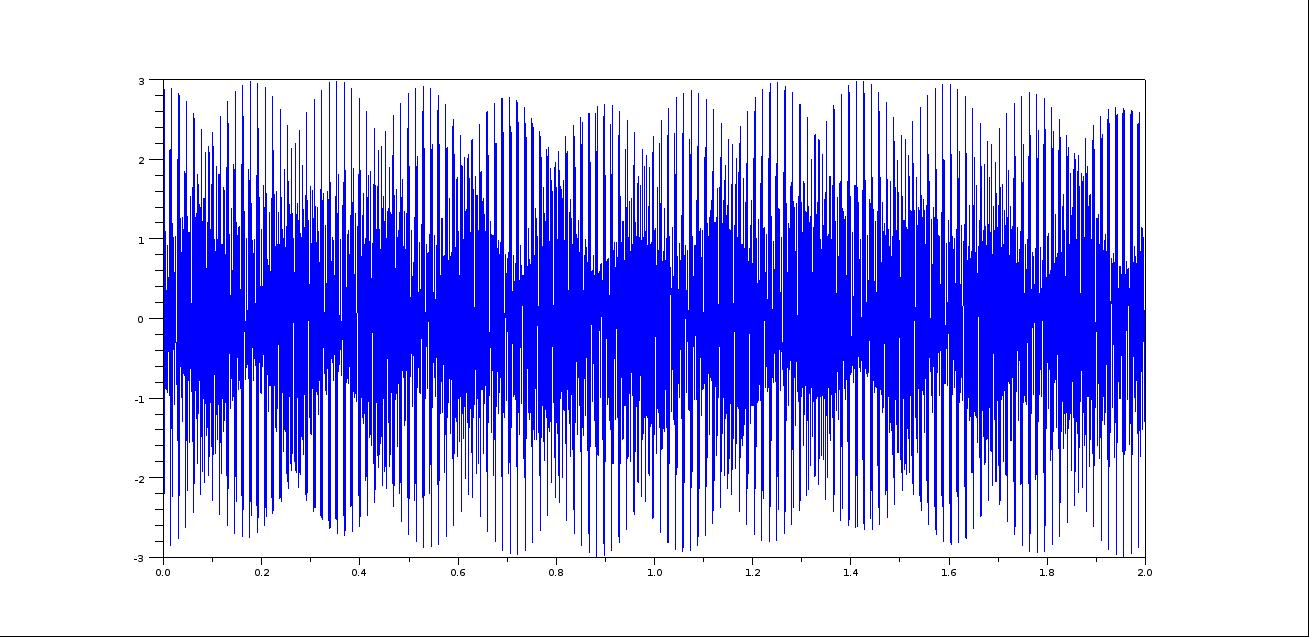
\includegraphics[width=\textwidth]{sumOfWav.jpg}
\caption{Sum of Wave}
\end{figure}

\subsection{6-second duration consecutive C, E, G notes}
\begin{gather}
rangeT = 22050 sample/second \times{} 6 second \times{} 0.0001 sample^{-1}\\
rangeT = 13.23
\end{gather}
\begin{lstlisting}[frame=single]
function y = sixSecond(t)
    y = (sin(261.63*2*%pi*t) .* Pi(1/4.41*t-0.5))
      + (sin(329.63*2*%pi*t) .* Pi(1/4.41*t-1.5))
      + (sin(392.00*2*%pi*t) .* Pi(1/4.41*t-2.5))
endfunction
t = 0 : 0.0001 : 13.23\end{lstlisting}
If sample interval is reduces to 0.01:
\begin{gather}
rangeT = 22050 sample/second \times{} 6 second \times{} 0.01 sample^{-1}\\
rangeT = 1323
\end{gather}
\begin{lstlisting}[frame=single]
function y= sixSecond2(t)
    y = (sin(261.63*2*%pi*t) .* Pi(1/441*t-0.5))
      + (sin(329.63*2*%pi*t) .* Pi(1/441*t-1.5))
      + (sin(392.00*2*%pi*t) .* Pi(1/441*t-2.5))
endfunction
t = 0 : 0.01 : 1323
\end{lstlisting}

\subsection{Question 5.3}
\textbf{Question 1:}\\
Play back the saved wave files using Windows Media player and comment on what you hear.\\
\textbf{Answer 1:}\\
The sound is simple and complete for middle C, sounds like phone busy sound.\\
The composited sound is noisy and sounds like \emph{BU-ZZZ}, but roughly the same pitch as middle C.\\
The 6-second duration sound like the output of simple piezo disc or simple buzzer, with 3 different tone. If sample interval is reduced to 0.01, the sound becomes sharper than before and the tones are decreased instead of increased.\\
\textbf{Question 2:}\\
Why do we need to use such a small sampling interval? What would happen if sampling interval is reduced to 0.01?\\
\textbf{Answer 2:}\\
Since the vector \emph{\textbf{t}} we are using is discrete, the wave we generated is basically the assembled dots connected with smooth wave lines. The wave sounds more real, since the dot are allocated more concentrated. If using 0.01 as first sampling interval and using 0.0001 as the second sampling interval, since we will generate two 6-second waves, the first one with wider sampling interval will return a higher frequency wave. A higher frequency wave sounds far differently from real sound and, because of higher frequency, the sound will have higher tones.

\section{Defining Delta Function and Verifying Its Properties}
Take use of the following method:\\ 
\begin{gather}
a\Pi{}(at) \xrightarrow{\scriptscriptstyle a\to\infty} \delta{}(t)
\end{gather}
\subsection{$\delta(t)$ and $e^t\delta(t-1)$}
\begin{lstlisting}[frame=single]
function y = delta(t)
    y = 200 * Pi(200 * t);
endfunction

function y = expDelta(t)
    y = %e^t .* delta(t - 1)
endfunction
\end{lstlisting}
\begin{figure}[H]
\centering
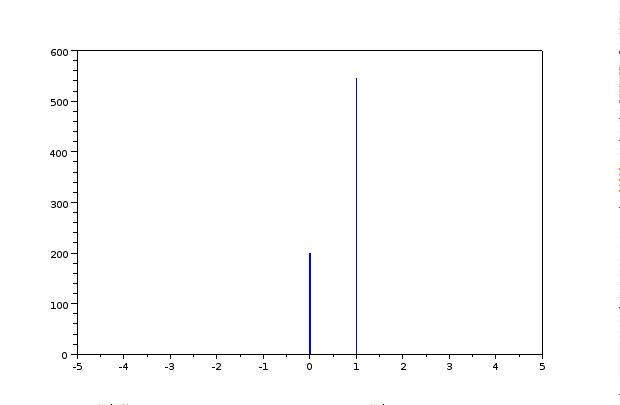
\includegraphics[width=\textwidth]{deltaAndEdelta.jpg}
\caption{$\delta(t)$ and $e^t\delta(t-1)$ (when $a = 200$)}
\end{figure}

\subsection{Evaluate $\int_0^2 e^t\delta(t-1)dt$}
\begin{figure}[H]
\centering
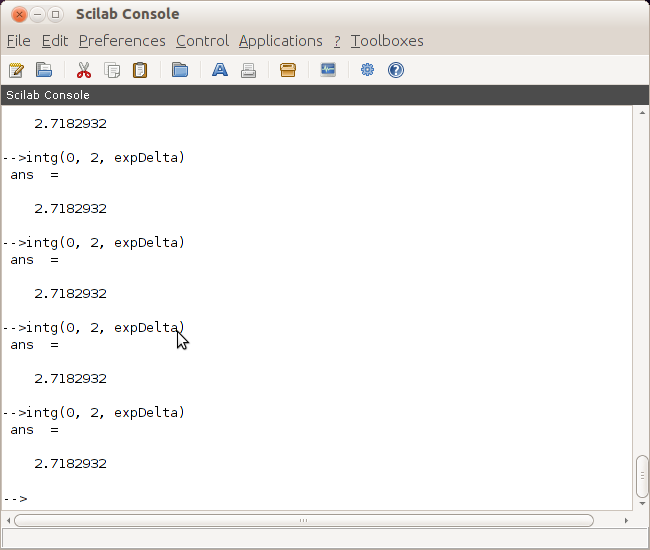
\includegraphics[width=\textwidth]{intgResult.png}
\caption{$\int_0^2 e^t \delta(t-1)dt$ result}
\end{figure}

\subsection{Question 5.4}
\textbf{Question:}\\
Save the plots and comment on the observed shapes and integration results using sampling and shifting property of the delta function.\\
\textbf{Answer:}\\
The value of \emph{\textbf{a}} is not supposed to be very large, otherwise, the value will be ignored due to precision issue.\\
The $e^t\delta(t-1)$ was generated by $\delta(t)$ through 1-unit right shifting and then lengthened its height to \emph{\textbf{e}} times than the original delta function.\\
Because the value of $\delta(t-1)$ equals to $\infty$ only when t = 1, otherwise 0; the integration $\int_0^2 e^t\delta(t-1)dt$ will only return the value of $e^t$ at $\delta(t-1)\neq 0$ . So the result is $e^t$ at $t=1$, which is \emph{\textbf{e}}.

\section{Signal Composition}
Define a function called square\underline{}series that is equal to $\sum_{k=1,k-odd}^n\frac{1}{k}sin(kt)$ .
\begin{lstlisting}[frame=single]
function y = kSumSin(k, t)
    y = 1/k * sin(k*t)
endfunction

function y = square_series(n, t)
    y = 0:0:0
    for i = 1 : 2 : n
        y = y + kSumSin(i, t)
    end
endfunction
\end{lstlisting}
\subsection{n = 1}
\begin{figure}[H]
\centering
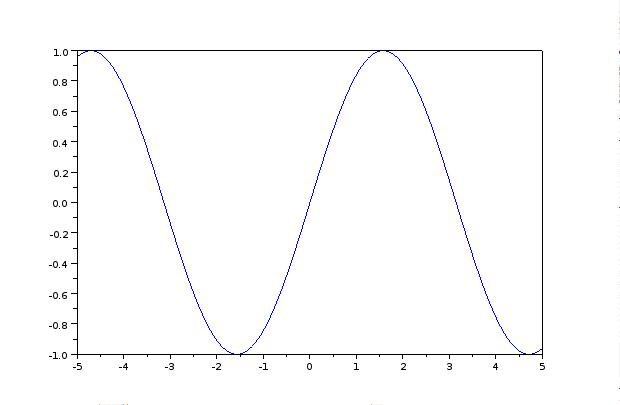
\includegraphics[width=.86\textwidth]{square_series1.jpg}
\caption{$sin(t)$}
\end{figure}

\subsection{n = 3}
\begin{figure}[H]
\centering
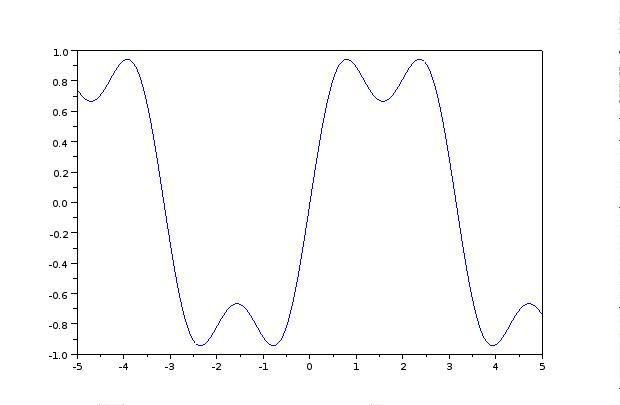
\includegraphics[width=.86\textwidth]{square_series3.jpg}
\caption{$\sum_{k=1,3}\frac{1}{k}sin(kt)$}
\end{figure}

\subsection{n = 9}
\begin{figure}[H]
\centering
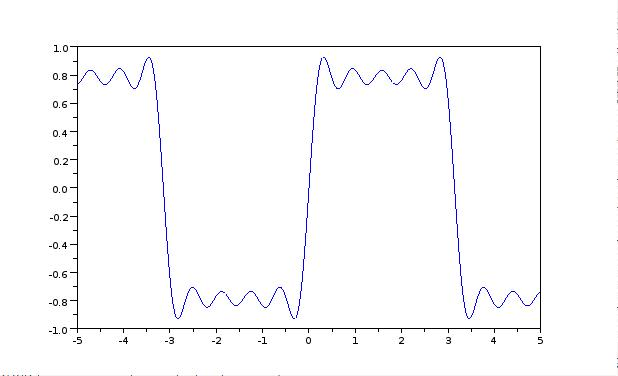
\includegraphics[width=\textwidth]{square_series9.jpg}
\caption{$\sum_{k=1,3,5,7,9}\frac{1}{k}sin(kt)$}
\end{figure}

\subsection{n = 100}
\begin{figure}[H]
\centering
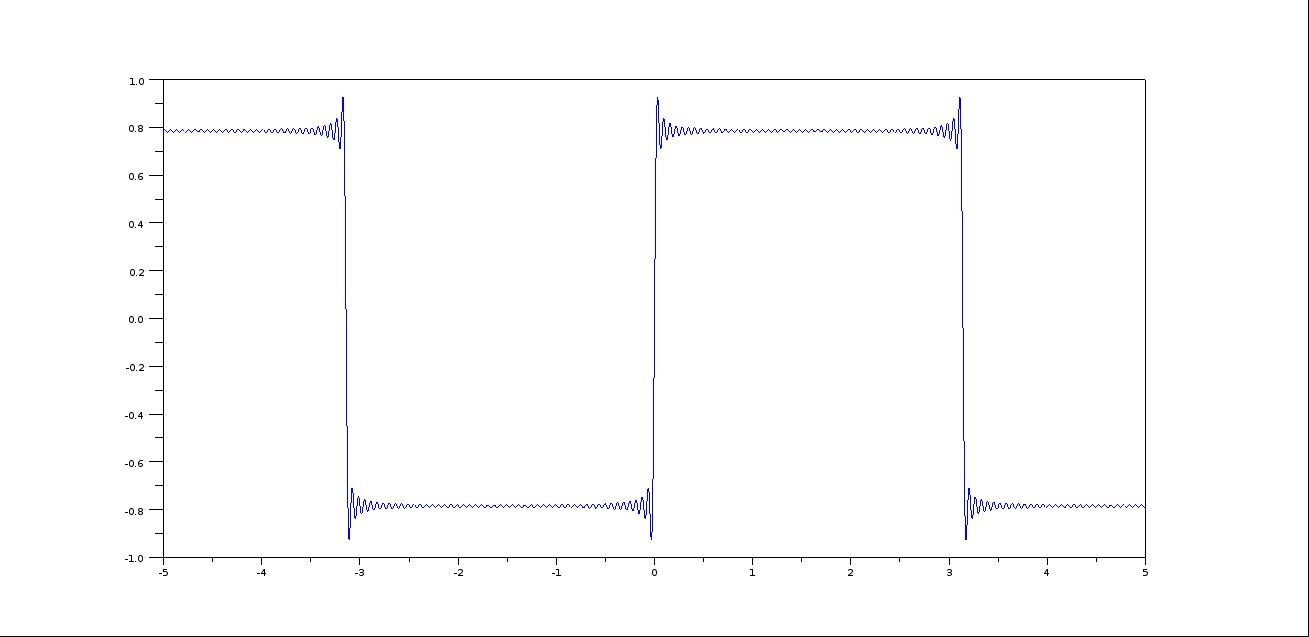
\includegraphics[width=\textwidth]{square_series100.jpg}
\caption{$\sum_{k=1,k-odd}^{100}\frac{1}{k}sin(kt)$}
\end{figure}
\subsection{Question 5.5}
\textbf{Question:}\\
Save the plots and comment on the shapes of observed signals.\\
\textbf{Answer:}\\
A set of sine waves are supposed to be able to generate a square wave according to trigonometric series:
\begin{gather}
\Pi(t) = sin\omega{}t+\frac{1}{3}sin3\omega{}t+\frac{1}{5}sin5\omega{}t+\cdots\\
\Leftrightarrow{}\Pi(t) =\sum_{k=1,k-odd}^n\frac{1}{k}sin(kt)
\end{gather}
When $n = 1$, the output is basically $sin(t)$ .\\
When $n = 3, 9$, the wave is an abstract square wave with unstable data at certain times.\\
When $n = 100$, the shape of square is already given, with unstable signal at both of the rising and dropping edges.\\
As \emph{\textbf{n}} goes bigger, the wave will be more accurate, which means it will looks and performs more similar to a square wave.
\end{document}
